\bta{共点力的平衡}

\begin{enumerate}
\renewcommand{\labelenumi}{\arabic{enumi}.}
% A(\Alph) a(\alph) I(\Roman) i(\roman) 1(\arabic)
%设定全局标号series=example	%引用全局变量resume=example
%[topsep=-0.3em,parsep=-0.3em,itemsep=-0.3em,partopsep=-0.3em]
%可使用leftmargin调整列表环境左边的空白长度 [leftmargin=0em]
\item
\exwhere{$ 2019 $年$ 4 $月浙江物理选考}
如图所示,一根粗糙的水平横杆上套有$ A $、$ B $两个轻环,系在两环上的登场细绳拴住的书本处于静止状态,现将两环距离变小后书本仍处于静止状态,则 \xzanswer{B} 



\begin{minipage}[h!]{0.7\linewidth}
\vspace{0.3em}
\fourchoices
{杆对$ A $环的支持力变大}
{$ B $环对杆的摩擦力变小}
{杆对$ A $环的力不变}
{与$ B $环相连的细绳对书本的拉力变大}

\vspace{0.3em}
\end{minipage}
\hfill
\begin{minipage}[h!]{0.3\linewidth}
\flushright
\vspace{0.3em}
\includesvg[width=0.6\linewidth]{picture/svg/430}
\vspace{0.3em}
\end{minipage}



\item 
\exwhere{$ 2019 $年物理天津卷}
$ 2018 $年$ 10 $月$ 23 $日,港珠澳跨海大桥正式通车。为保持以往船行习惯,在航道处建造了单面索(所有钢索均处在同一竖直面内)斜拉桥,其索塔与钢索如图所示。下列说法正确的是 \xzanswer{C} 
\begin{figure}[h!]
\centering
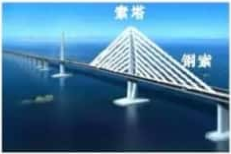
\includegraphics[width=0.23\linewidth]{picture/Picture1.png}
\end{figure}



\fourchoices
{增加钢索的数量可减小索塔受到的向下的压力}
{为了减小钢索承受拉力,可以适当降低索塔的高度}
{索塔两侧钢索对称且拉力大小相同时,钢索对索塔的合力竖直向下}
{为了使索塔受到钢索的合力竖直向下,索塔两侧的钢索必须对称分布}




\item 
\exwhere{$ 2019 $年物理全国\lmd{3}卷}
用卡车运输质量为$ m $的匀质圆筒状工件,为使工件保持固定,将其置于两光滑斜面之间,如图所示。两斜面 \lmd{1} 、 \lmd{2} 固定在车上,倾角分别为$ 30 ^{ \circ } $和$ 60 ^{ \circ } $。重力加速度为$ g $。当卡车沿平直公路匀速行驶时,圆筒对斜面 \lmd{1} 、 \lmd{2} 压力的大小分别为$ F_{1} $、$ F_{2} $,则 \xzanswer{D} 
\begin{figure}[h!]
\centering
\includesvg[width=0.23\linewidth]{picture/svg/433}
\end{figure}

\fourchoices
{$ F _ { 1 } = \frac { \sqrt { 3 } } { 3 } m g , F _ { 2 } = \frac { \sqrt { 3 } } { 2 } m g $}
{$ F _ { 1 } = \frac { \sqrt { 3 } } { 2 } m g , F _ { 2 } = \frac { \sqrt { 3 } } { 3 } m g $}
{$ F _ { 1 } = \frac { 1 } { 2 } m g , F _ { 2 } = \frac { \sqrt { 3 } } { 2 } m g $}
{$ F _ { 1 } = \frac { \sqrt { 3 } } { 2 } m g , \quad F _ { 2 } = \frac { 1 } { 2 } m g $}

\item 
\exwhere{$ 2019 $年物理江苏卷}
如图所示,一只气球在风中处于静止状态,风对气球的作用力水平向右.细绳与竖直方向的夹角为$ \alpha $,绳的拉力为$ T $,则风对气球作用力的大小为 \xzanswer{C} 


\begin{minipage}[h!]{0.7\linewidth}
\vspace{0.3em}
\fourchoices
{$\frac { T } { \sin \alpha } \quad$}
{$\frac { T } { \cos \alpha } \quad$}
{$T \sin \alpha \quad$}
{$T \cos \alpha$}

\vspace{0.3em}
\end{minipage}
\hfill
\begin{minipage}[h!]{0.3\linewidth}
\flushright
\vspace{0.3em}
\includesvg[width=0.5\linewidth]{picture/svg/434}
\vspace{0.3em}
\end{minipage}


\item 
\exwhere{$ 2019 $年物理全国\lmd{1}卷}
如图,一粗糙斜面固定在地面上,斜面顶端装有一光滑定滑轮。一细绳跨过滑轮,其一端悬挂物块$ N $。另一端与斜面上的物块$ M $相连,系统处于静止状态。现用水平向左的拉力缓慢拉动$ N $,直至悬挂$ N $的细绳与竖直方向成$ 45 ^{ \circ } $。已知$ M $始终保持静止,则在此过程中 \xzanswer{BD} 
\begin{figure}[h!]
\centering
\includesvg[width=0.23\linewidth]{picture/svg/435}
\end{figure}



\fourchoices
{水平拉力的大小可能保持不变}
{$ M $所受细绳的拉力大小一定一直增加}
{$ M $所受斜面的摩擦力大小一定一直增加}
{$ M $所受斜面的摩擦力大小可能先减小后增加}




\item 
\exwhere{$ 2012 $年理综广东卷}
如图所示,两根等长的轻绳将日光灯悬挂在天花板上,两绳与竖直方向的夹角都为$ 45 ^{ \circ } $,日光灯保持水平,所受重力为$ G $,左右两绳的拉力大小分别为 \xzanswer{B} 
\begin{figure}[h!]
\centering
\includesvg[width=0.23\linewidth]{picture/svg/437}
\end{figure}

\fourchoices
{$ G $和$ G $ }
{$ \frac{\sqrt{2}}{2} G $和$ \dfrac{\sqrt{2}}{2} G $}
{$ \frac{ 1 }{ 2 } G $ 和$ \dfrac{\sqrt{3}}{2} G $}
{$ \frac{ 1 }{ 2 } G $和$ \frac{ 1 }{ 2 } G $}


\item 
\exwhere{$ 2012 $年理综新课标卷}
如图,一小球放置在木板与竖直墙面之间。设墙面对球的压力大小为$ N_{1} $,球对木板的压力大小为$ N_{2} $。以木板与墙连接点所形成的水平直线为轴,将木板从图示位置开始缓慢地转到水平位置。不计摩擦,在此过程中 \xzanswer{B} 

\begin{minipage}[h!]{0.7\linewidth}
\vspace{0.3em}
\fourchoices
{$ N_{1} $始终减小,$ N_{2} $始终增大}
{$ N_{1} $始终减小,$ N_{2} $始终减小}
{$ N_{1} $先增大后减小,$ N_{2} $始终减小}
{$ N_{1} $先增大后减小,$ N_{2} $先减小后增大}

\vspace{0.3em}
\end{minipage}
\hfill
\begin{minipage}[h!]{0.3\linewidth}
\flushright
\vspace{0.3em}
\includesvg[width=0.3\linewidth]{picture/svg/438}
\vspace{0.3em}
\end{minipage}


\item 
\exwhere{$ 2013 $年天津卷}
如图所示,小球用细绳系住,绳的另一端固定于$ O $点。现用水平力$ F $缓慢推动斜面体,小球在斜面上无摩擦地滑动,细绳始终处于直线状态,当小球升到接近斜面顶端时细绳接近水平,此过程中斜面对小球的支持力$ F_{N} $以及绳对小球的拉力$ F_T $的变化情况是 \xzanswer{D} 
\begin{figure}[h!]
\centering
\includesvg[width=0.23\linewidth]{picture/svg/439}
\end{figure}


\fourchoices
{$ F_{N} $保持不变,$ F_T $不断增大}
{$ F_{N} $不断增大,$ F_T $不断减小}
{$ F_{N} $保持不变,$ F_T $先增大后减小}
{$ F_{N} $不断增大,$ F_T $先减小后增大}



\item 
\exwhere{$ 2012 $年理综浙江卷}
如图所示,与水平面夹角为$ 30 ^{ \circ } $的固定斜面上有一质量$ m=1.0 \ kg $的物体。细绳的一端与物体相连,另一端经摩擦不计的定滑轮与固定的弹簧秤相连。物体静止在斜面上,弹簧秤的示数为$ 4.9 \ N $。关于物体受力的判断(取$ g=9.8 \ m/s ^{2} $),下列说法正确的是 \xzanswer{A} 
\begin{figure}[h!]
\centering
\includesvg[width=0.23\linewidth]{picture/svg/440}
\end{figure}


\fourchoices
{斜面对物体的摩擦力大小为零}
{斜面对物体的摩擦力大小为$ 4.9 \ N $,方向沿斜面向上}
{斜面对物体的支持力大小为$ N $,方向竖直向上}
{斜面对物体的支持力大小为$ 4.9 \ N $,方向垂直斜面向上}



\item 
\exwhere{$ 2011 $年理综安徽卷}
一质量为$ m $的物块恰好静止在倾角为$ \theta $的斜面上。现对物块施加一个竖直向下的恒力$ F $,如图所示。则物块 \xzanswer{A} 
\begin{figure}[h!]
\centering
\includesvg[width=0.23\linewidth]{picture/svg/441}
\end{figure}


\fourchoices
{仍处于静止状态}
{沿斜面加速下滑}
{受到的摩擦力不便}
{受到的合外力增大}


\item 
\exwhere{$ 2014 $年物理上海卷}
如图,光滑的四分之一圆弧轨道$ AB $固定在竖直平面内,$ A $端与水平面相切。穿在轨道上的小球在拉力$ F $作用下,缓慢地由$ A $向$ B $运动,$ F $始终沿轨道的切线方向,轨道对球的弹力为$ N $。在运动过程中 \xzanswer{A} 

\begin{minipage}[h!]{0.7\linewidth}
\vspace{0.3em}
\fourchoices
{$ F $增大,$ N $减小 }
{$ F $减小,$ N $减小}
{$ F $增大,$ N $增大 }
{$ F $减小,$ N $增大}


\vspace{0.3em}
\end{minipage}
\hfill
\begin{minipage}[h!]{0.3\linewidth}
\flushright
\vspace{0.3em}
\includesvg[width=0.6\linewidth]{picture/svg/442}
\vspace{0.3em}
\end{minipage}	

\item 
\exwhere{$ 2011 $年海南卷}
如图,墙上有两个钉子$ a $和$ b $,它们的连线与水平方向的夹角为$ 45 ^{ \circ } $,两者的高度差为$ l $。一条不可伸长的轻质细绳一端固定于$ a $点,另一端跨过光滑钉子$ b $悬挂一质量为$ m_{1} $的重物。在绳子距$ a $端$ l/2 $的$ c $点有一固定绳圈。若绳圈上悬挂质量为$ m_{2} $的钩码,平衡后绳的$ ac $段正好水平,则重物和钩码的质量比$ m_{1} / m_{2} $为 \xzanswer{C} 

\begin{minipage}[h!]{0.7\linewidth}
\vspace{0.3em}
\fourchoices
{$ \sqrt { 5 } $}
{$ 2 $}
{$ \frac { \sqrt { 5 } } { 2 } $}
{$ \sqrt { 2 } $}
\vspace{0.3em}
\end{minipage}
\hfill
\begin{minipage}[h!]{0.3\linewidth}
\flushright
\vspace{0.3em}
\includesvg[width=0.5\linewidth]{picture/svg/443}
\vspace{0.3em}
\end{minipage}

\item 
\exwhere{$ 2014 $年物理海南卷}
如图,一不可伸长的光滑轻绳,其左端固定于$ O $点,右端跨过位于$ O ^{\prime} $点的固定光滑轴悬挂一质量为$ M $的物体;$ OO ^{\prime} $ 段水平,长为度$ L $;绳上套一可沿绳滑动的轻环。现在轻环上悬挂一钩码,平衡后,物体上升$ L $。则钩码的质量为 \xzanswer{D} 

\begin{minipage}[h!]{0.7\linewidth}
\vspace{0.3em}
\fourchoices
{$\frac { \sqrt { 2 } } { 2 } M \quad$}
{$\frac { \sqrt { 3 } } { 2 } M $}
{$ \sqrt { 2 } M $}
{$ \sqrt { 3 } M$	}

\vspace{0.3em}
\end{minipage}
\hfill
\begin{minipage}[h!]{0.3\linewidth}
\flushright
\vspace{0.3em}
\includesvg[width=0.5\linewidth]{picture/svg/444}
\vspace{0.3em}
\end{minipage}
\item 
\exwhere{$ 2014 $年理综新课标 \lmd{1} 卷}
如图,用橡皮筋将一小球悬挂在小车的架子上,系统处于平衡状态。现使小车从静止开始向左加速,加速度从零开始逐渐增大到某一值,然后保持此值,小球稳定地偏离竖直方向某一角度(橡皮筋在弹性限度内 )。与稳定在竖直位置时相比,小球高度 \xzanswer{A} 
\begin{figure}[h!]
\centering
\includesvg[width=0.16\linewidth]{picture/svg/445}
\end{figure}


\fourchoices
{一定升高}
{一定降低}
{保持不变}
{升高或降低由橡皮筋的劲度系数决定}



\item 
\exwhere{$ 2012 $年理综山东卷}
如图所示,两相同轻质硬杆$ OO_{1} $、$ OO_{2} $可绕其两端垂直纸面的水平轴$ O $、$ O_{1} $、$ O_{2} $转动,在$ O $点悬挂一重物$ M $,将两相同木块$ m $紧压在竖直挡板上,此时整个系统保持静止。$ F_f $表示木块与挡板间摩擦力的大小,$ F_{N} $表示木块与挡板间正压力的大小。若挡板间的距离稍许增大后,系统仍静止且$ O_{1} $、$ O_{2} $始终等高,则 \xzanswer{BD} 
\begin{figure}[h!]
\centering
\includesvg[width=0.25\linewidth]{picture/svg/446}
\end{figure}

\fourchoices
{$ F_f $ 变小}
{$ F_f $ 不变}
{$ F_{N} $ 变小}
{$ F_{N} $ 变大}


\item 
\exwhere{$ 2017 $年新课标 \lmd{1} 卷}
如图,柔软轻绳$ ON $的一端$ O $固定,其中间某点$ M $拴一重物,用手拉住绳的另一端$ N $,初始时,$ OM $竖直且$ MN $被拉直,$ OM $与$ MN $之间的夹角为$ \alpha $($ \alpha
>\frac{\pi}{2} $)。现将重物向右上方缓慢拉起,并保持夹角$ \alpha
$不变。在$ OM $由竖直被拉到水平的过程中 \xzanswer{AD} 
\begin{figure}[h!]
\centering
\includesvg[width=0.13\linewidth]{picture/svg/447}
\end{figure}


\fourchoices
{$ MN $上的张力逐渐增大}
{$ MN $上的张力先增大后减小}
{$ OM $上的张力逐渐增大}
{$ OM $上的张力先增大后减小}


\item 
\exwhere{$ 2017 $年新课标 \lmd{2} 卷}
如图,一物块在水平拉力$ F $的作用下沿水平桌面做匀速直线运动。若保持$ F $的大小不变,而方向与水平面成$ 60 ^{ \circ } $角,物块也恰好做匀速直线运动。物块与桌面间的动摩擦因数为 \xzanswer{C} 
\begin{figure}[h!]
\centering
\includesvg[width=0.23\linewidth]{picture/svg/448}
\end{figure}

\fourchoices
{$ 2 - \sqrt { 3 } $}
{$ \frac { \sqrt { 3 } } { 6 } $}
{$ \frac { \sqrt { 3 } } { 3 } $}
{$ \frac { \sqrt { 3 } } { 2 } $}


\item 
\exwhere{$ 2017 $年新课标 \lmd{3} 卷}
一根轻质弹性绳的两端分别固定在水平天花板上相距$ 80 \ cm $的两点上,弹性绳的原长也为$ 80 \ cm $。将一钩码挂在弹性绳的中点,平衡时弹性绳的总长度为$ 100 \ cm $;再将弹性绳的两端缓慢移至天花板上的同一点,则弹性绳的总长度变为(弹性绳的伸长始终处于弹性限度内) \xzanswer{B} 


\fourchoices
{$ 86 \ cm $}
{$ 92 \ cm $}
{$ 98 \ cm $ }
{$ 104 \ cm $}

\item 
\exwhere{$ 2016 $年新课标 \lmd{2} 卷}
质量为$ m $的物体用轻绳$ AB $悬挂于天花板上。用水平向左的力$ F $缓慢拉动绳的中点$ O $,如图所示。用$ T $ 表示绳$ OA $段拉力的大小,在$ O $点向左移动的过程中 \xzanswer{A} 
\begin{figure}[h!]
\centering
\includesvg[width=0.16\linewidth]{picture/svg/449}
\end{figure}


\fourchoices
{$ F $逐渐变大,$ T $逐渐变大}
{$ F $逐渐变大,$ T $逐渐变小}
{$ F $逐渐变小,$ T $逐渐变大}
{$ F $逐渐变小,$ T $逐渐变小}


\newpage	

\item 
\exwhere{$ 2017 $年天津卷}
如图所示,轻质不可伸长的晾衣绳两端分别固定在竖直杆$ M $、$ N $上的$ a $、$ b $两点,悬挂衣服的衣架钩是光滑的,挂于绳上处于静止状态。如果只人为改变一个条件,当衣架静止时,下列说法正确的是 \xzanswer{AB} 
\begin{figure}[h!]
\centering
\includesvg[width=0.23\linewidth]{picture/svg/450}
\end{figure}


\fourchoices
{绳的右端上移到$ b‘	 $,绳子拉力不变}
{将杆$ N $向右移一些,绳子拉力变大}
{绳的两端高度差越小,绳子拉力越小}
{若换挂质量更大的衣服,则衣服架悬挂点右移}



\item 
\exwhere{$ 2011 $年物理江苏卷}
如图所示,石拱桥的正中央有一质量为$ m $的对称楔形石块,侧面与竖直方向的夹角为$ \alpha $,重力加速度为$ g $。若接触面间的摩擦力忽略不计,则石块侧面所受弹力的大小为 \xzanswer{A} 
\begin{figure}[h!]
\centering
\includesvg[width=0.33\linewidth]{picture/svg/451}
\end{figure}

\fourchoices
{$ \frac { m g } { 2 \sin \alpha } $}
{$ \frac { m g } { 2 \cos \alpha } $}
{$ \frac { 1 } { 2 } m g \tan \alpha $}
{$ \frac { 1 } { 2 } m g \cot \alpha $}




\item 
\exwhere{$ 2015 $年上海卷}
如图,一质量为$ m $的正方体物块置于风洞内的水平面上,其一面与风速垂直,当风速为$ v_{0} $时刚好能推动该物块。已知风对物块的推力$ F \propto Sv^2 $,其中$ v $为风速、$ S $为物块迎风面积。当风速变为$ 2v_0 $时,刚好能推动用同一材料做成的另一正方体物块,则该物块的质量为 \xzanswer{D} 


\begin{minipage}[h!]{0.7\linewidth}
\vspace{0.3em}
\fourchoices
{$ 4 \ m $}
{$ 8 \ m $}
{$ 32 \ m $}
{$ 64 \ m $}
\vspace{0.3em}
\end{minipage}
\hfill
\begin{minipage}[h!]{0.3\linewidth}
\flushright
\vspace{0.3em}
\includesvg[width=0.6\linewidth]{picture/svg/452}
\vspace{0.3em}
\end{minipage}


\item 
\exwhere{$ 2016 $年新课标 \lmd{3} 卷}
如图,两个轻环$ a $和$ b $套在位于竖直面内的一段固定圆弧上;一细线穿过两轻环,其两端各系一质量为$ m $的小球。在$ a $和$ b $之间的细线上悬挂一小物块。平衡时,$ a $、$ b $间的距离恰好等于圆弧的半径。不计所有摩擦。小物块的质量为 \xzanswer{C} 
\begin{figure}[h!]
\centering
\includesvg[width=0.23\linewidth]{picture/svg/453}
\end{figure}


\fourchoices
{$ \frac { m } { 2 } $}
{$ \frac { \sqrt { 3 } } { 2 } m $}
{$ m $}
{$ 2 m $}




\item 
\exwhere{$ 2016 $年新课标 \lmd{1} 卷}
如图,一光滑的轻滑轮用细绳$ OO ^{\prime} $ 悬挂于点;另一细绳跨过滑轮,其一端悬挂物块$ a $,另一端系一位于水平粗糙桌面上的物块$ b $。外力向右上方拉$ b $,整个系统处于静止状态。若$ F $方向不变,大小在一定范围内变化,物块$ b $仍始终保持静止,则 \xzanswer{BD} 
\begin{figure}[h!]
\centering
\includesvg[width=0.23\linewidth]{picture/svg/455}
\end{figure}


\fourchoices
{绳$ OO ^{\prime} $的张力也在一定范围内变化}
{物块$ b $所受到的支持力也在一定范围内变化}
{连接$ a $和$ b $的绳的张力也在一定范围内变化}
{物块$ b $与桌面间的摩擦力也在一定范围内变化}




\item 
\exwhere{$ 2012 $年理综新课标卷}
拖把是由拖杆和拖把头构成的擦地工具(如图)。设拖把头的质量为$ m $,拖杆质量可以忽略;拖把头与地板之间的动摩擦因数为常数$ \mu $,重力加速度为$ g $,某同学用该拖把在水平地板上拖地时,沿拖杆方向推拖把,拖杆与竖直方向的夹角为$ \theta $。
\begin{enumerate}
\renewcommand{\labelenumii}{(\arabic{enumii})}

\item 
若拖把头在地板上匀速移动,求推拖把的力的大小。

\item 
设能使该拖把在地板上从静止刚好开始运动的水平推力与此时地板对拖把的正压力的比值为λ。已知存在一临界角$ \theta _0 $,若$ \theta \leq \theta _ 0 $,则不管沿拖杆方向的推力多大,都不可能使拖把从静止开始运动。求这一临界角的正切$ \tan \theta _0 $。
\end{enumerate}
\begin{figure}[h!]
\flushright
\includesvg[width=0.25\linewidth]{picture/svg/454}
\end{figure}

\banswer{

}



\newpage	
\item 
\exwhere{$ 2013 $年福建卷}
质量为$ M $、长为$ \sqrt{3}L $的杆水平放置,杆两端$ A $、$ B $系着长为$ 3L $的不可伸长且光滑的柔软轻绳,绳上套着一质量为$ m $的小铁环。已知重力加速度为$ g $,不计空气影响。
\begin{enumerate}
\renewcommand{\labelenumi}{\arabic{enumi}.}
% A(\Alph) a(\alph) I(\Roman) i(\roman) 1(\arabic)
%设定全局标号series=example	%引用全局变量resume=example
%[topsep=-0.3em,parsep=-0.3em,itemsep=-0.3em,partopsep=-0.3em]
%可使用leftmargin调整列表环境左边的空白长度 [leftmargin=0em]
\item
现让杆和环均静止悬挂在空中,如图甲,求绳中拉力的大小;
\item 
若杆与环保持相对静止,在空中沿$ AB $方向水平向右做匀加速直线运动,此时环恰好悬于$ A $端的正下方,如图乙所示。

①求此状态下杆的加速度大小$ a $;

②为保持这种状态需在杆上施加一个多大的外力,方向如何?



\end{enumerate}
\begin{figure}[h!]
\flushright
\includesvg[width=0.25\linewidth]{picture/svg/456} \qquad \qquad 
\includesvg[width=0.25\linewidth]{picture/svg/457}	
\end{figure}

\banswer{

}




\end{enumerate}










